\appendix
\section{SPICE - ISO/IEC 15504}  \label{spice}
L'\glo{ISO/IEC 15504}, noto come progetto \glo{\textit{SPICE}} (Software Process Improvement and Capability Evaluation), ha come obiettivo quello di sviluppare uno \glo{standard} che consenta valutazioni omogenee di organizzazioni software allo scopo di:
\begin{itemize}
	\item Identificare i punti forti, i punti deboli e i rischi delle metodologie utilizzate;
	\item Individuare le situazioni nelle quali le metodologie utilizzate permettono di raggiungere in maniera \glo{efficace} gli obiettivi prefissati.
\end{itemize}
Per effettuare la classificazione dei diversi processi, viene valutato e attribuito loro un livello di \textit{Capability}, cioè la capacità di essere cognitivamente capace di raggiungere il suo scopo. 
Ogni livello comprende degli attributi sui quali effettuare la valutazione.
I livelli considerati con i loro attributi sono i seguenti:
\begin{itemize}
	\item \textbf{Livello 0 Incomplete}: il processo non è implementato e non è in grado di raggiungere gli obiettivi;
	\item \textbf{Livello 1 Performed}: il processo è implementato e raggiunge gli obiettivi ma non è sottoposto a controlli costanti ai fini di correzione e miglioramento.
	Attributi associati:
	\begin{itemize}
		\item \textbf{Performance di Processo (PP)}: numero degli obiettivi raggiunti.
	\end{itemize}
	\item \textbf{Livello 2 Managed}: il processo è gestito tramite pianificazione, controllo e correzione, l'output raggiunge gli obiettivi fissati.
	Attributi associati:
	\begin{itemize}
		\item \textbf{Gestione delle performance (PM)}: grado di organizzazione degli obiettivi fissati;
		\item \textbf{Gestione del prodotto di lavoro (WPM)}: grado di organizzazione dei \glo{prodotti} rilasciati.
	\end{itemize}
	\item \textbf{Livello 3 Established}: esiste un'insieme di standard per il processo.
	Attributi associati:
	\begin{itemize}
		\item \textbf{Definizione di processo (PDEF)}: grado di adesione del processo agli standard;
		\item \textbf{Rilascio di processo (PDEP)}: grado di misura della garanzia di rilascio con reperibilità.
	\end{itemize}
	\item \textbf{Livello 4 Predictable}: il processo è istanziato coerentemente rispetto ai limiti previsti, è quantitativamente misurato per assicurarne il mantenimento delle performance.
	Attributi associati:
	\begin{itemize}
		\item \textbf{Misurazioni di processo (PME)}: misura con quanta \glo{efficacia} le metriche possono essere applicate al processo;
		\item \textbf{Controllo di processo (PC)}: grado di predicibilità dei risultati delle valutazioni.
	\end{itemize}
	\item \textbf{Livello 5 Innovating}: il processo migliora attraverso feedback quantitativi e gli standard sono adattati di conseguenza.
	Attributi associati:
	\begin{itemize}
		\item \textbf{Innovazione di processo (PI)}: misura quanto i cambiamenti attuati nel processo siano innovativi e positivi;
		\item \textbf{Ottimizzazione di processo (PO)}: misura quanto la curva di miglioramento sia lineare.
	\end{itemize}
\end{itemize}
Ogni attributo viene valutato e ad esso viene assegnato uno dei seguenti livelli, a seconda del grado di soddisfazione dello stesso:
\begin{itemize}
	\item \textbf{N not achieved}: 0\%-15\%, il processo non ha implementato l'attributo o presenta gravi lacune;
	\item \textbf{P partially achieved}: 16\%-50\%, il processo ha implementato l'attributo in modo sistematico ma risulta migliorabile o poco predicibile;
	\item \textbf{L largely achieved}: 51\%-85\%, il processo ha ampiamente implementato l'attributo ma il suo valore è poco uniforme rispetto alle altri parti del processo;
	\item \textbf{F fully achieved}: 86\%-100\%, il processo ha implementato completamente l'attributo ed è uniforme in ogni sua parte.
\end{itemize}

\newpage

\section{Ciclo di Deming - PDCA} \label{PDCA}
Il ciclo \glo{\textit{PDCA}} è un metodo iterativo con l'obiettivo di stabilire un modello per il miglioramento continuo dei processi ed essere garanzia di \glo{qualità} \glo{efficiente} e continuativa. 
A tal fine si individuano quattro passaggi:
\begin{itemize}
	\item\textbf{Plan}: pianificazione, si esamina la situazione attuale al fine di determinare esattamente come raggiungere l'obiettivo;
	\item\textbf{Do}: implementazione, si procede a piccoli passi per realizzare quanto previsto durante la pianificazione;
	\item\textbf{Check}: verifica, vengono raccolti i risultati ottenuti e valutati rispetto agli obiettivi prefissati;
	\item\textbf{Act}: azione, i problemi e le cause identificate vengono risolte adattando quanto pianificato e infine attuato.
\end{itemize}
\begin{center}
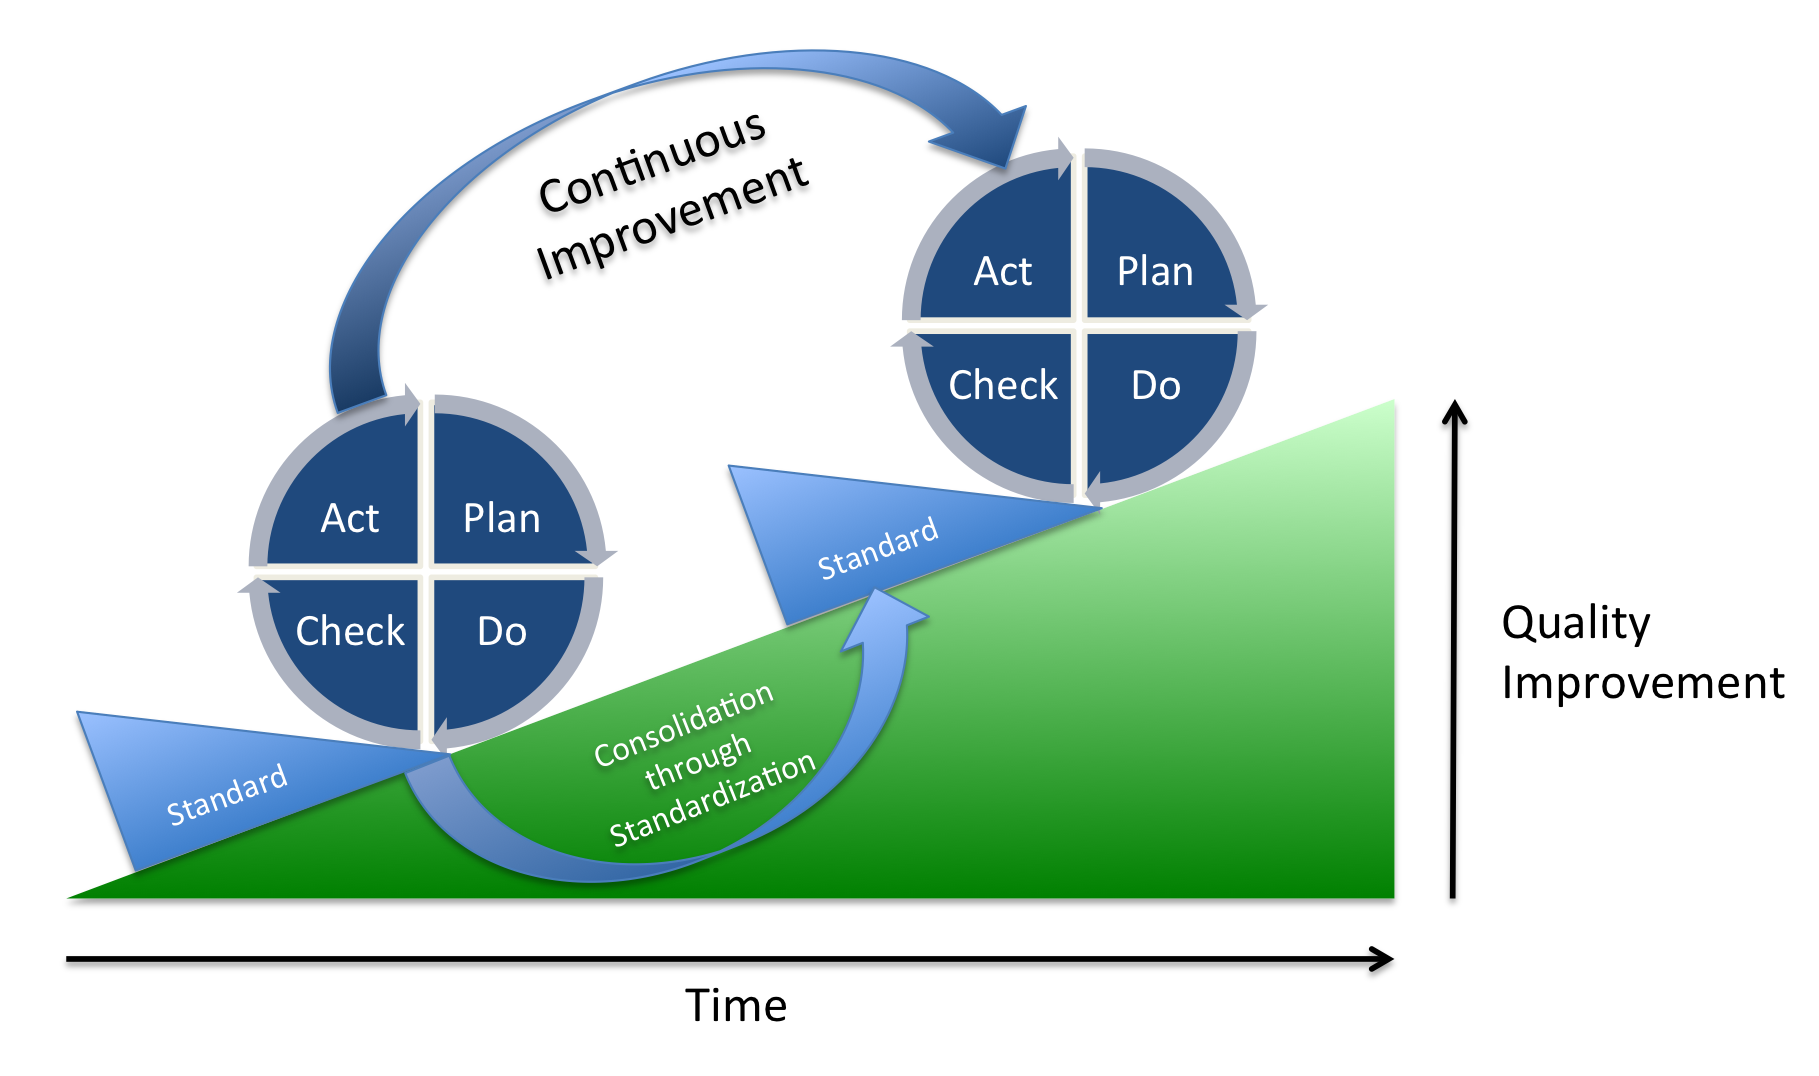
\includegraphics[scale=0.25]{Immagini/PDCA.png}
\captionof{figure}{Ciclo di Deming}
\end{center}

\newpage
\section{Standard ISO/IEC 9126}\label{9126}
L'\glo{ISO/IEC 9126} è uno standard internazionale per la valutazione della qualità del software, le norme presenti definiscono le caratteristiche che la determinano e propongono metriche per la misurazione.
Il modello di qualità software stabilito dallo standard considera sei caratteristiche principali da soddisfare, ovvero:
\begin{itemize}
	\item \textbf{Funzionalità};
	\item \textbf{Affidabilità};
	\item \textbf{Efficienza};
	\item \textbf{Usabilità};
	\item \textbf{Manutenibilità};
	\item \textbf{Portabilità}.
\end{itemize}
Le caratteristiche elencate possono essere misurate da \textit{metriche esterne}, \textit{metriche interne} e \textit{metriche per la qualità d'uso}.
\paragraph*{Metriche Esterne}
Misurano i comportamenti del prodotto software rilevabili dai \glo{test}, dall'operatività e dall'osservazione durante la sua esecuzione, in funzione degli obiettivi stabiliti. 
\paragraph*{Metriche Interne}
Si applicano alla documentazione e al prodotto non eseguibile, ad esempio il codice sorgente, durante la progettazione e la codifica. Queste metriche misurano attributi interni del software e forniscono indicazioni sulle caratteristiche esterne del prodotto finale individuando problemi che potrebbero ridurne la qualità.
\paragraph*{Metriche per la qualità d'uso}
Misurano il grado con cui il prodotto software permette agli utenti di svolgere le proprie attività con efficacia, produttività, soddisfazione e sicurezza.

\section{Metriche} \label{Metriche}
\subsection{Metriche per la qualità del processo}
Di seguito sono elencate le metriche utilizzate per misurare il raggiungimento degli obiettivi della qualità di processo.
\subsubsection{MPR01: Budget at Completion}
Rappresenta il valore previsto per la realizzazione del progetto secondo quanto previsto nel \PdPv{1.0.0}.
\subsubsection{MPR02: Actual Cost of Work Performed}
Corrisponde alla somma di tutte le spese sostenute dal gruppo fino al momento in cui l'indice viene calcolato, il limite superiore dipende da quanto stabilito nel \glo{Preventivo} presente nel \PdPv{1.0.0}.
\subsubsection{MPR03: Budget Cost of Work Performed}
Valore intero effettivo del prodotto ottenuto fino al momento in cui l'indice viene calcolato.
\subsubsection{MPR04: Budget Cost of Work Scheduled}
Valore intero corrispondente alla spesa pianificata per l'attività di progetto alla data corrente, reperibile nel \glo{Preventivo} presente nel \PdPv{1.0.0}.
\subsubsection{MPR05: Schedule Variance}
Indica se si è in linea, in anticipo o in ritardo rispetto alla schedulazione delle attività di progetto pianificate nella \glo{baseline}.\\
Viene calcolato nel seguente modo:
\begin{center}
	\textbf{SV = BCWP – BCWS}
\end{center}
dove 
\begin{itemize}
	\item \textbf{BCWP} sta per \textit{Budgeted Cost of Work Performed};
	\item \textbf{BCWS} sta per \textit{Budgeted Cost of Work Scheduled}.
\end{itemize}
In base al risultato ottenuto abbiamo:
\begin{itemize}
	\item \textbf{SV>0}: il gruppo sta producendo con maggior velocità rispetto quanto pianificato;
	\item \textbf{SV=0}: il gruppo sta producendo secondo quanto pianificato;
	\item \textbf{SV<0}: il gruppo sta producendo con minor velocità rispetto quanto pianificato, è necessaria un revisione di quanto pianificato.
\end{itemize}
\subsubsection{MPR06: Budget Variance}
Indica se il gruppo rientra nel budget di spesa previsto alla data corrente.\\
Viene calcolato nel seguente modo:
\begin{center}
	\textbf{BV = BCWS – ACWP}
\end{center}
dove
\begin{itemize}
	\item \textbf{BCWS} sta per \textit{Budgeted Cost of Work Scheduled};
	\item \textbf{ACWP} sta per \textit{Actual Cost of Work Performed}.
\end{itemize}
Un valore positivo segnala che i costi sostenuti rientrano nel budget preventivato.
\subsubsection{MPR07: Soddisfacimento Requisiti Obbligatori}
Indica la percentuale di requisiti obbligatori soddisfatti nel momento in cui viene calcolato.\\
Viene calcolato nel seguente modo:
\begin{center}
	\textbf{RO=\(\frac{ROC}{RO}\)*100}
\end{center}
dove
\begin{itemize}
	\item \textbf{RO} sta per \textit{Requisiti Obbligatori};
	\item \textbf{ROC} sta per \textit{Requisiti Obbligatori Coperti dall'implementazione}.
\end{itemize}
\subsubsection{MPR08: Indice di Gulpease}
L'indice permette di stabilire la difficoltà di lettura di un testo.\\
Viene calcolato nel seguente modo:
\begin{center}
	\(
	GULP = 89+\frac{300\times\# frasi-10\times\#lettere}{\#parole}
	\)
\end{center}
L'indice può assumere i seguenti valori:
\begin{itemize}
	\item \textbf{GULP<80}: indica una leggibilità difficile per un utente con licenza elementare;
	\item \textbf{GULP<60}: indica una leggibilità difficile per un utente con licenza media;
	\item \textbf{GULP<40}: indica una leggibilità difficile per un utente con licenza superiore.
\end{itemize}
\subsubsection{MPR09: Indice di correttezza ortografica}
Indica la correttezza ortografica in un documento.\\
Viene calcolato nel seguente modo:
\begin{center}
	\textbf{CORT = \# numero di errori ortografici}
\end{center}
Un risultato maggiore di zero indica la presenza di errori nel documento.
\subsubsection{MPR10: Indice di risoluzione dei problemi}
L'indice calcola la velocità con cui le \glo{issue} vengono risolte, viene calcolata la media dei numeri di giorni che intercorrono tra l'apertura e la chiusura per ogni issue.

\subsection{Metriche per la qualità di prodotto}
Di seguito sono elencate le metriche utilizzate per misurare il raggiungimento degli obiettivi della qualità di prodotto.
\subsubsection{MPDS01: Completezza dell'implementazione}
L'indice stabilisce la completezza del prodotto software realizzato nel momento in cui viene calcolato rispetto a tutti i requisiti previsti dall'\AdRv{1.0.0}.\\
Viene calcolato nel seguente modo:
\begin{center}
	\textbf{CI=\(1-\frac{FNI}{FI}\)*100}
\end{center}
dove
\begin{itemize}
	\item \textbf{FNI} indica il numero di funzionalità non implementate;
	\item \textbf{FI} indica il numero di funzionalità implementate.
\end{itemize}
\subsubsection{MPDS02: Densità errori}
Rappresenta la percentuale di righe di codice che possono causare errori.\\
Viene calcolato nel seguente modo:
\begin{center}
	\textbf{DE=\(\frac{RB}{RTOT}\)*100}
\end{center}
dove
\begin{itemize}
	\item \textbf{RB} indica il numero di linee di codice che possono causare imprevisti o comportamenti diversi da quelli desiderati;
	\item \textbf{RTOT} indica il numero di linee di codice totali.
\end{itemize}
\subsubsection{MPDS03: Facilità di utilizzo}
Il valore stabilisce la semplicità per un utente di raggiungere quanto cercato valutando il numero di click medio per raggiungere il contenuto desiderato.
\subsubsection{MPDS04: Facilità di apprendimento}
Il valore stabilisce la semplicità per un utente di raggiungere quanto cercato all'interno del sito calcolando la media dei minuti necessari per raggiungere le pagine ricercate.
\subsubsection{MPDS05:  Profondità della gerarchia}
Il valore risultante viene calcolato individuando la profondità media delle pagine rispetto alla home page.
\subsubsection{MPDS06: Facilità di comprensione}
Il valore indica la facilità di comprensione del codice in base al numero di righe di commento presenti.\\
Viene calcolato nel seguente modo:
\begin{center}
	\textbf{FC=\(\frac{LCOM}{LCOD}\)*100}
\end{center}
dove
\begin{itemize}
	\item \textbf{LCOM} indica il numero di linee di commento;
	\item \textbf{LCOD} indica il numero di linee di codice.
\end{itemize}
\subsubsection{MPDS07: Semplicità delle funzioni}
Il valore stabilisce la semplicità di un metodo basandosi sul numero di parametri a lui necessari.
\subsubsection{MPDS08: Semplicità delle classi}
Il valore stabilisce la semplicità di una classe basandosi sul numero di metodi al suo interno.